\documentclass[notes,11pt, aspectratio=169]{beamer}

\usepackage{pgfpages}
% These slides also contain speaker notes. You can print just the slides,
% just the notes, or both, depending on the setting below. Comment out the want
% you want.
\setbeameroption{hide notes} % Only slide
%\setbeameroption{show only notes} % Only notes
%\setbeameroption{show notes on second screen=right} % Both

\usepackage{helvet}
\usepackage[default]{lato}
\usepackage{array}
\usepackage{tgbonum}

\usepackage{tikz}
\usepackage{verbatim}
\setbeamertemplate{note page}{\pagecolor{yellow!5}\insertnote}
\usetikzlibrary{positioning}
\usetikzlibrary{snakes}
\usetikzlibrary{calc}
\usetikzlibrary{arrows}
\usetikzlibrary{decorations.markings}
\usetikzlibrary{shapes.misc}
\usetikzlibrary{matrix,shapes,arrows,fit,tikzmark}
\usepackage{amsmath}
\usepackage{mathpazo}
\usepackage{hyperref}
\usepackage{lipsum}
\usepackage{multimedia}
\usepackage{graphicx}
\usepackage{multirow}
\usepackage{graphicx}
\usepackage{dcolumn}
\usepackage{bbm}
\newcolumntype{d}[0]{D{.}{.}{5}}

\usepackage{changepage}
\usepackage{appendixnumberbeamer}
\newcommand{\beginbackup}{
   \newcounter{framenumbervorappendix}
   \setcounter{framenumbervorappendix}{\value{framenumber}}
   \setbeamertemplate{footline}
   {
     \leavevmode%
     \hline
     box{%
       \begin{beamercolorbox}[wd=\paperwidth,ht=2.25ex,dp=1ex,right]{footlinecolor}%
%         \insertframenumber  \hspace*{2ex} 
       \end{beamercolorbox}}%
     \vskip0pt%
   }
 }
\newcommand{\backupend}{
   \addtocounter{framenumbervorappendix}{-\value{framenumber}}
   \addtocounter{framenumber}{\value{framenumbervorappendix}} 
}


\usepackage{graphicx}
\usepackage[space]{grffile}
\usepackage{booktabs}
\newcommand\independent{\protect\mathpalette{\protect\independenT}{\perp}}
\def\independenT#1#2{\mathrel{\rlap{$#1#2$}\mkern2mu{#1#2}}}
\DeclareMathOperator{\Supp}{Supp}


\newtheorem{assN}{Assumption}
% These are my colors -- there are many like them, but these ones are mine.
\definecolor{blue}{RGB}{0,114,178}
\definecolor{red}{RGB}{213,94,0}
\definecolor{yellow}{RGB}{240,228,66}
\definecolor{green}{RGB}{0,158,115}

\hypersetup{
  colorlinks=false,
  linkbordercolor = {white},
  linkcolor = {blue}
}


%% I use a beige off white for my background
\definecolor{MyBackground}{RGB}{255,253,218}

%% Uncomment this if you want to change the background color to something else
%\setbeamercolor{background canvas}{bg=MyBackground}

%% Change the bg color to adjust your transition slide background color!
\newenvironment{transitionframe}{
  \setbeamercolor{background canvas}{bg=yellow}
  \begin{frame}}{
    \end{frame}
}

\setbeamercolor{frametitle}{fg=blue}
\setbeamercolor{title}{fg=black}
\setbeamertemplate{footline}[frame number]
\setbeamertemplate{navigation symbols}{} 
\setbeamertemplate{itemize items}{-}
\setbeamercolor{itemize item}{fg=blue}
\setbeamercolor{itemize subitem}{fg=blue}
\setbeamercolor{enumerate item}{fg=blue}
\setbeamercolor{enumerate subitem}{fg=blue}
\setbeamercolor{button}{bg=MyBackground,fg=blue,}



% If you like road maps, rather than having clutter at the top, have a roadmap show up at the end of each section 
% (and after your introduction)
% Uncomment this is if you want the roadmap!
% \AtBeginSection[]
% {
%    \begin{frame}
%        \frametitle{Roadmap of Talk}
%        \tableofcontents[currentsection]
%    \end{frame}
% }
\setbeamercolor{section in toc}{fg=blue}
\setbeamercolor{subsection in toc}{fg=red}
\setbeamersize{text margin left=1em,text margin right=1em} 

\newenvironment{wideitemize}{\itemize\addtolength{\itemsep}{10pt}}{\enditemize}

\usepackage{environ}
\NewEnviron{videoframe}[1]{
  \begin{frame}
    \vspace{-8pt}
    \begin{columns}[onlytextwidth, T] % align columns
      \begin{column}{.70\textwidth}
        \begin{minipage}[t][\textheight][t]
          {\dimexpr\textwidth}
          \vspace{8pt}
          \hspace{4pt} {\Large \sc \textcolor{blue}{#1}}
          \vspace{8pt}
          
          \BODY
        \end{minipage}
      \end{column}%
      \hfill%
      \begin{column}{.38\textwidth}
        \colorbox{green!20}{\begin{minipage}[t][1.2\textheight][t]
            {\dimexpr\textwidth}
            Face goes here
          \end{minipage}}
      \end{column}%
    \end{columns}
  \end{frame}
}

\title[]{\textcolor{blue}{Supervised Machine Learning III: \\ Unstructured and Unsupervised ML}} \author[PGP]{}
\institute[FRBNY]{\small{\begin{tabular}{c}
                           Paul Goldsmith-Pinkham  \\
\end{tabular}}}

\date{\today}

\begin{document}

%%% TIKZ STUFF
\tikzset{   
        every picture/.style={remember picture,baseline},
        every node/.style={anchor=base,align=center,outer sep=1.5pt},
        every path/.style={thick},
        }
\newcommand\marktopleft[1]{%
    \tikz[overlay,remember picture] 
        \node (marker-#1-a) at (-.3em,.3em) {};%
}
\newcommand\markbottomright[2]{%
    \tikz[overlay,remember picture] 
        \node (marker-#1-b) at (0em,0em) {};%
}
\tikzstyle{every picture}+=[remember picture] 
\tikzstyle{mybox} =[draw=black, very thick, rectangle, inner sep=10pt, inner ysep=20pt]
\tikzstyle{fancytitle} =[draw=black,fill=red, text=white]
%%%% END TIKZ STUFF

% Title Slide
\begin{frame}
\maketitle
\end{frame}

\begin{frame}{Unstructured Data and Unsupervised Learning}
  \begin{wideitemize}
  \item We have, so far, discussed ML in the context of two assumptions:
    \begin{enumerate}
    \item Our data was a relatively well-defined (\emph{feature} matrix $X$ and outcome $y$)
    \item We had an outcome ($y$) to go with each set of predictors
    \end{enumerate}
  \item Today we'll talk about settings where these are relaxed
  \item Data that is 
    \begin{itemize}
    \item unstructured (e.g. some data $\mathcal{X}$ that we need to turn into a matrix $X$)
    \item unlabeled (no outcome $y$ defined)
    \end{itemize}
  \item The key challenge with this literature is keeping eye on the prize:
    \begin{itemize}
    \item Our goal is to answer \emph{economic} questions
    \end{itemize}
  \end{wideitemize}
\end{frame}

\begin{frame}{Huge space of tools}
  \only<1>{  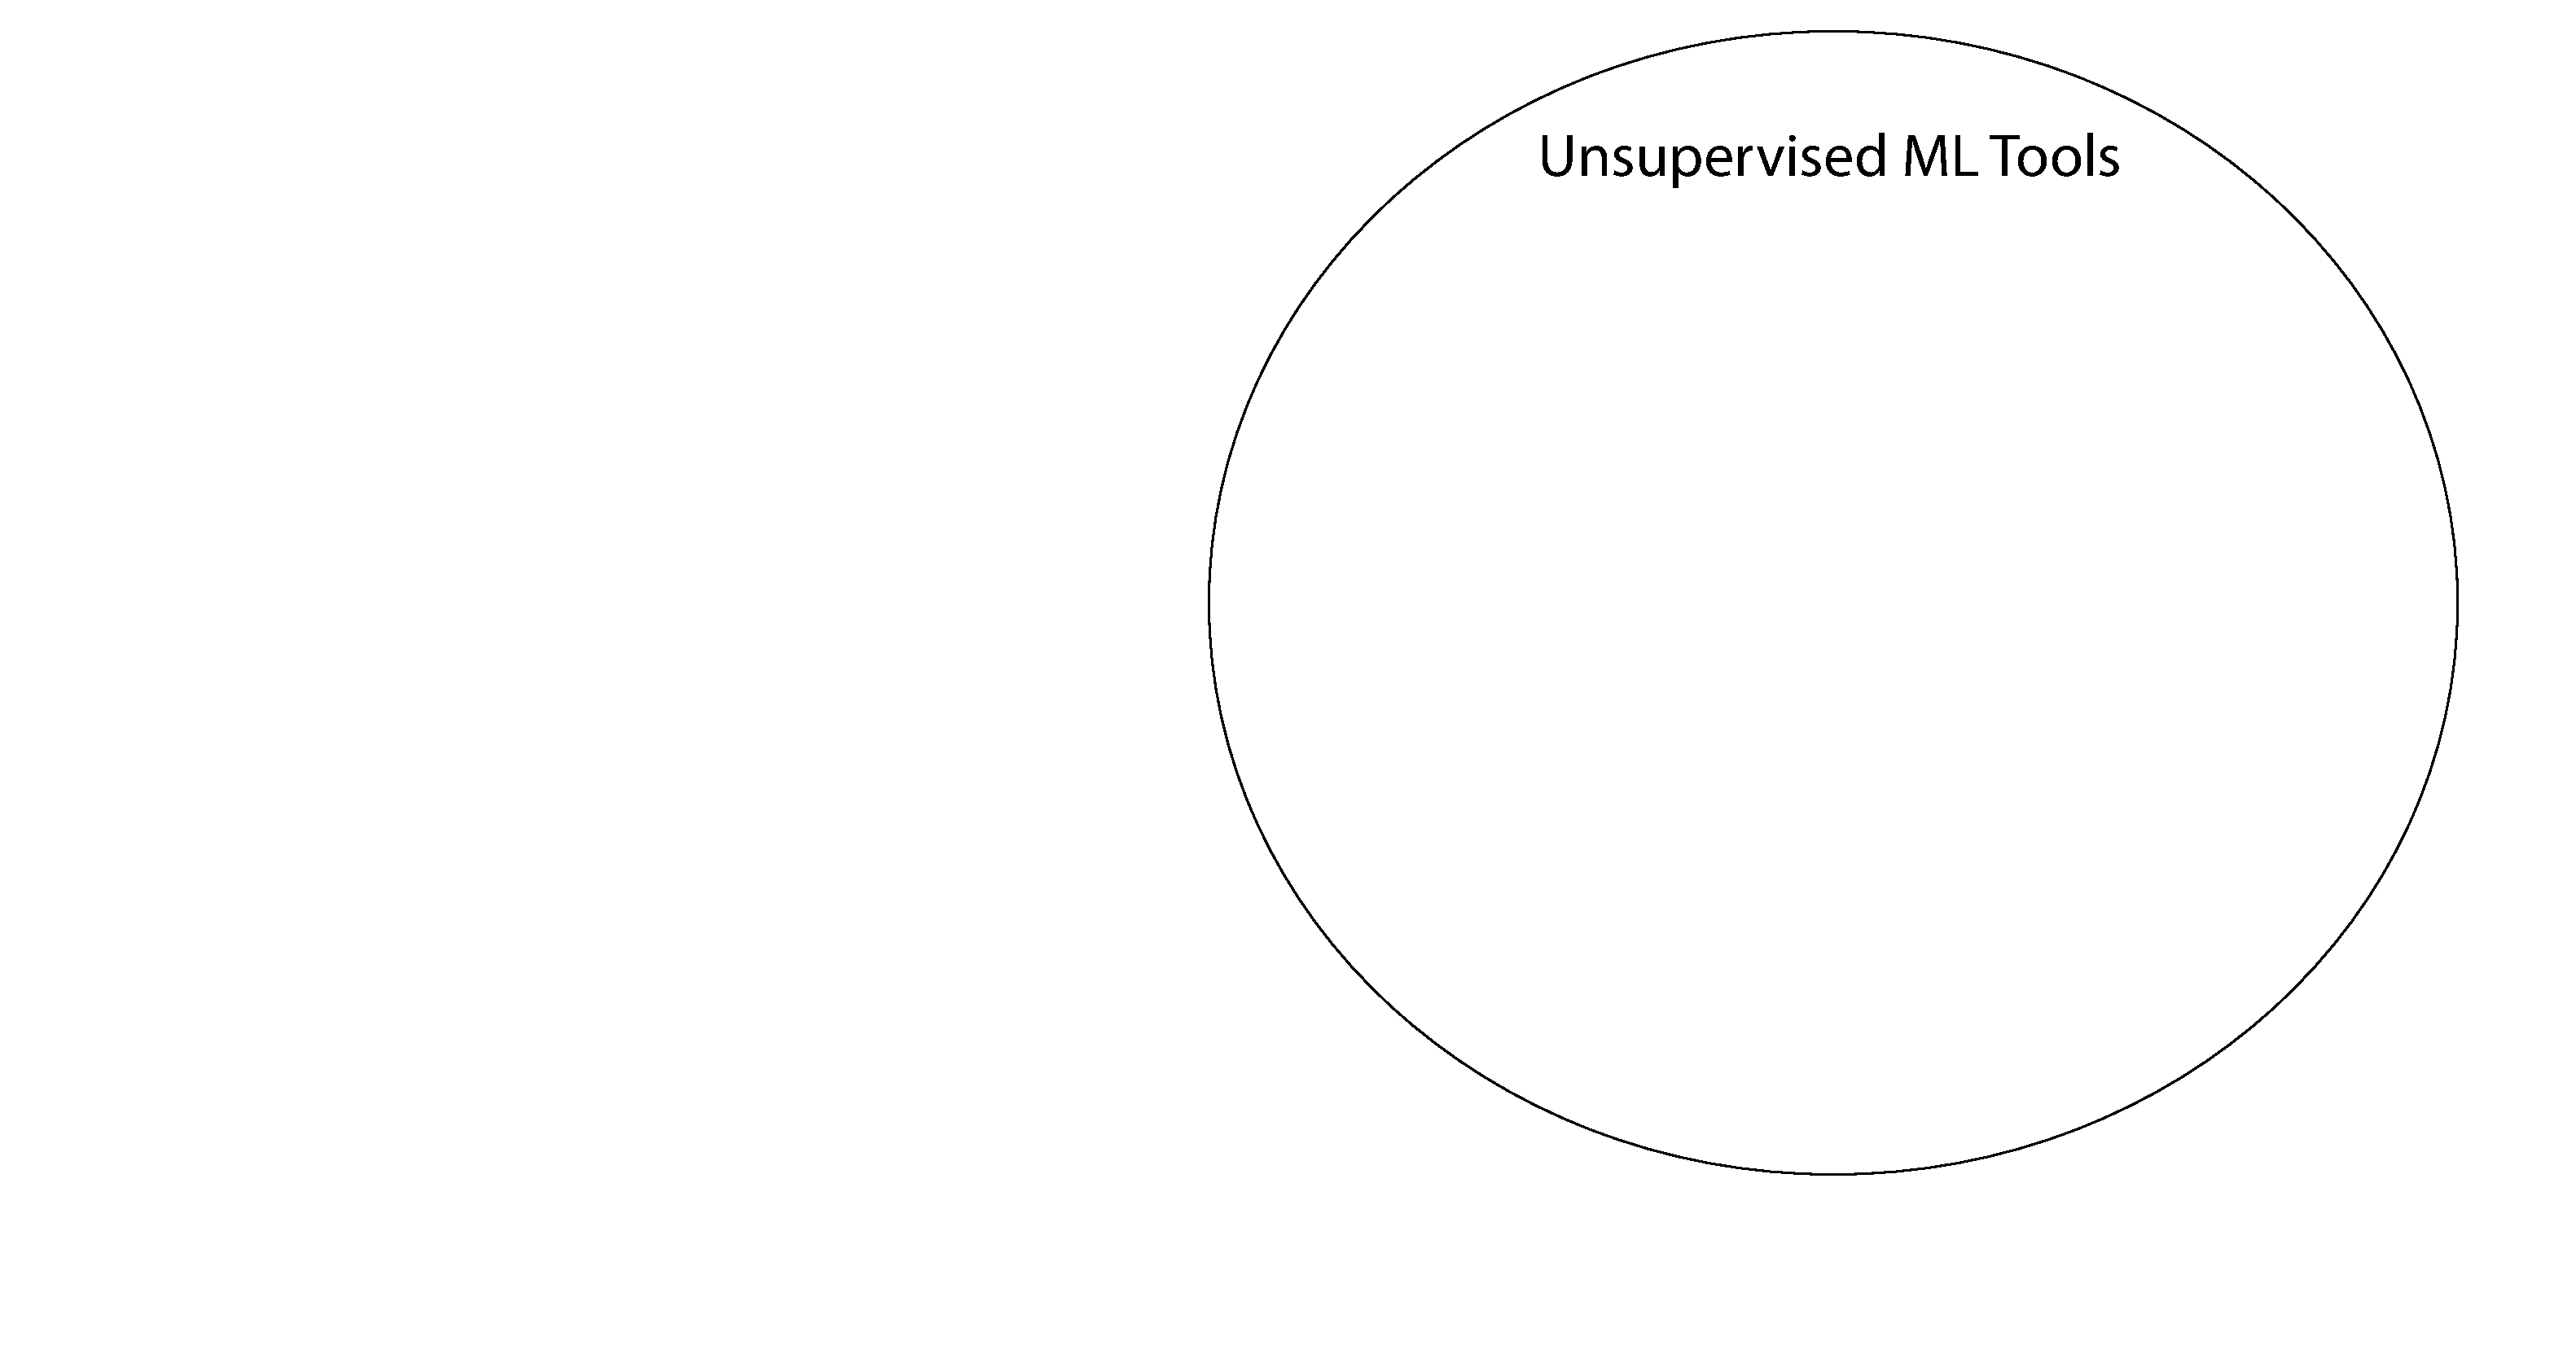
\includegraphics[width=\linewidth]{images/unsupervisedml_venn2.pdf}}
\only<2>{  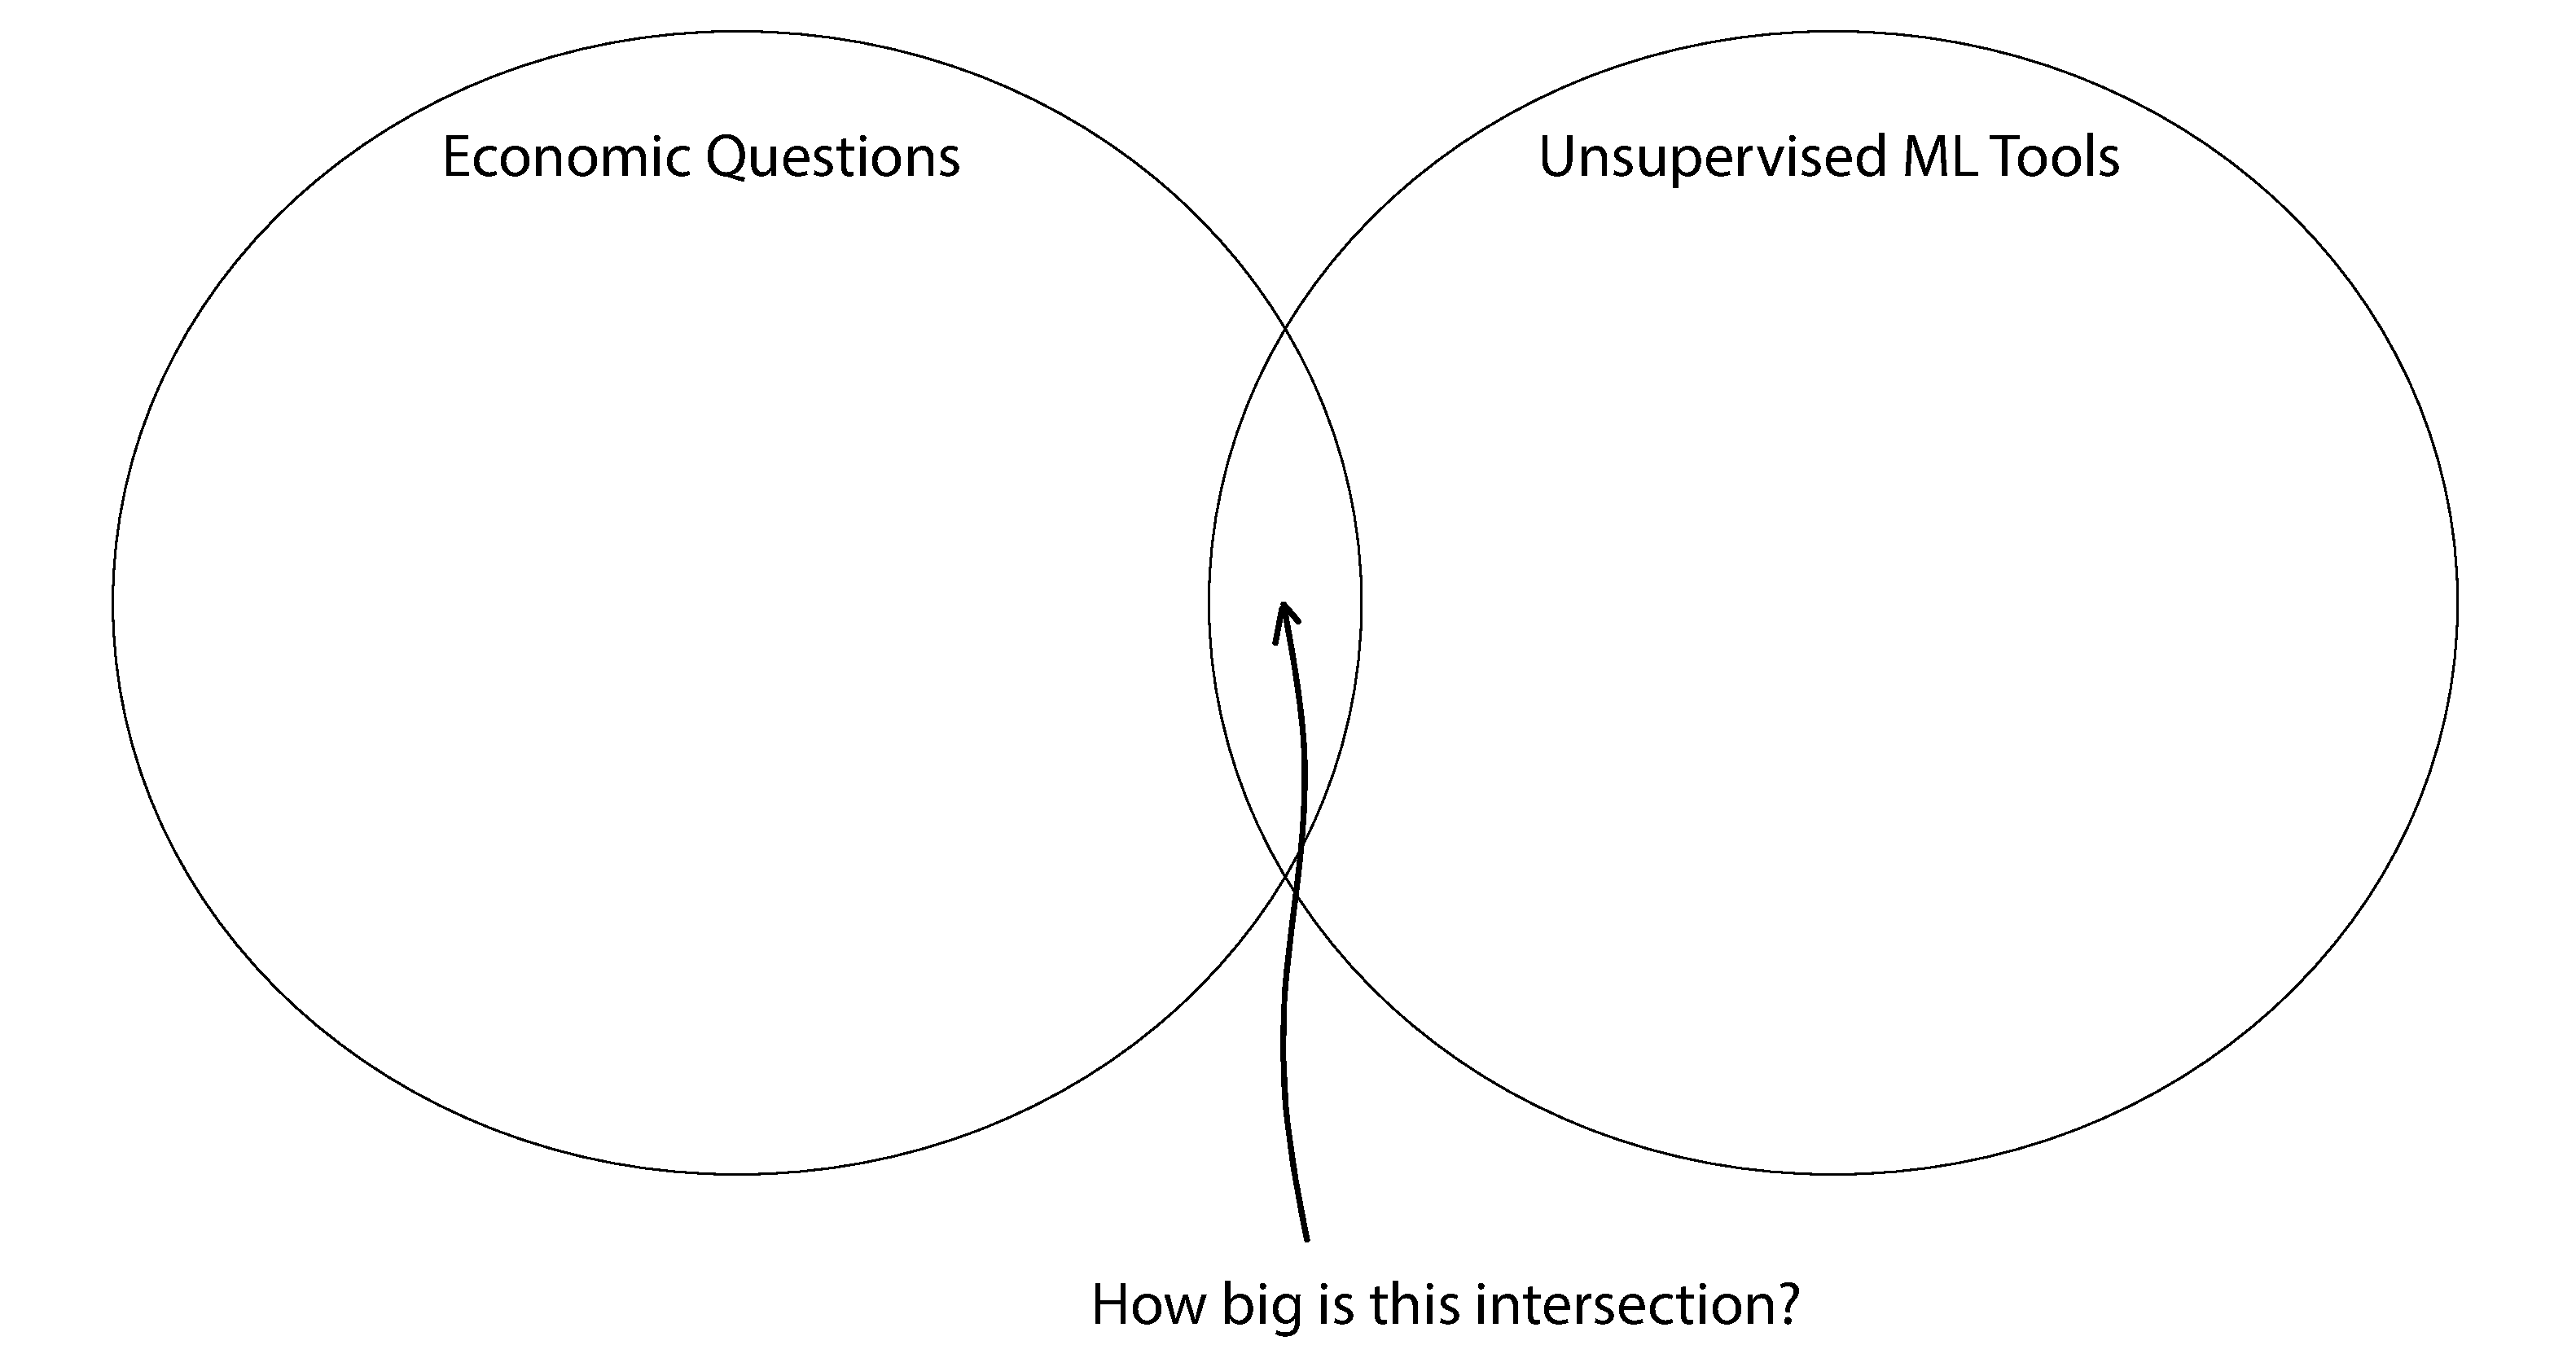
\includegraphics[width=\linewidth]{images/unsupervisedml_venn.pdf}}  
\end{frame}

\begin{frame}{Some high level notation}
  \begin{wideitemize}
  \item Consider a data object $\mathcal{X}$ which is complex and challenging to describe
    \begin{itemize}
    \item A set of firms or products with various characteristics
    \item The collection of news articles over time 
    \item Evaluations of banks' health
    \item A set of congressional speeches
    \item Etc.
    \end{itemize}
  \item First step in the process is a mapping, $\psi(\mathcal{X}) \rightarrow X$
    \begin{itemize}
    \item This typically involves some sort of quantification
    \item This also include the construction or addition of a label, $y$ that goes along with the data
      \begin{itemize}
      \item This will give the data a supervised ML structure
      \end{itemize}
    \item This object will likely be very high dimensional! (e.g. $dim(X_{i}) >$ observations)
    \end{itemize}
  \item Next step in the process: constructing economic masures or features from $X$
    \begin{itemize}
    \item Calculating ``interesting'' subdimensions of $X$ (summarization )
    \item Projecting labels $y$ onto dimensions of $X$
    \item Projecting units into new dimensions based on $X$ (e.g. relative distance metrics)
    \end{itemize}
  \item Will provide examples for each case...
  \end{wideitemize}
\end{frame}


\begin{frame}{Today's Class}
      \begin{columns}[onlytextwidth, T] % align columns
      \begin{column}{.9\textwidth}
        \begin{wideitemize}
        \item A  overview of two different examples /
          applications where unusual unstructured data was used
        \item A brief dive into one particular unsupervised ML technique, Latent Dirichlet Allocation (LDA)
          \begin{itemize}
          \item Commonly used in text data (things with counts)
          \end{itemize}
        \item Goal: highlight that these techniques can be very powerful at unlocking new measures
          \begin{itemize}
          \item But they require \emph{extremely} judicious selection of applications / approaches 
          \end{itemize}
        \item What I want you to avoid is a common situation (that I have been in):
          \begin{itemize}
          \item ``Amazing data in search of a question'' (a real quote
            from one of my advisors)
          \end{itemize}
        \end{wideitemize}
      \end{column}%
      \hfill%
      \begin{column}{.5\textwidth}
      \end{column}%
    \end{columns}
\end{frame}

\begin{frame}{Example 1: Gentzkow and Shapiro (2010)}
      \begin{columns}[onlytextwidth, T] % align columns
      \begin{column}{.5\textwidth}
        \begin{wideitemize}
        \item How do we evaluate the ``slant'' of a newspaper?
          \begin{itemize}
          \item Subjective: go through and label yourself (or get others)
          \end{itemize}
        \item $\mathcal{X}$ is the ``newspaper'' and ``politics''
          \begin{itemize}
          \item $X$ is now two sets of data:
          \item $X_{1}$ - text from newspapers
          \item $X_{2}$ - text from congressional speakers
          \item $Y_{2}$ - \emph{labels} of political party
          \end{itemize}
        \item How are $X_{1}$ and $X_{2}$ constructed? 
        \end{wideitemize}
      \end{column}%
      \hfill%
      \begin{column}{.5\textwidth}
        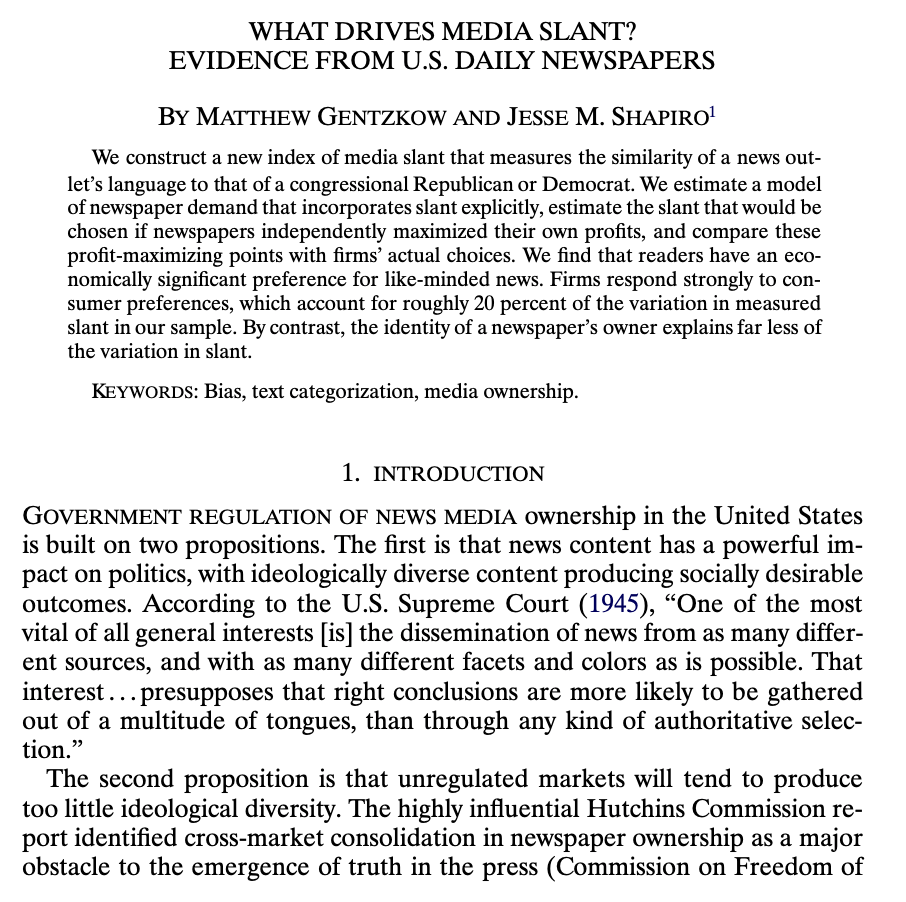
\includegraphics[width=\linewidth]{images/gentzkowshapiro_1.png}
      \end{column}%
    \end{columns}
\end{frame}

\begin{frame}{Aside on quantifying text data }
  \begin{wideitemize}
  \item Given a \emph{corpus} of text, this unstructured data can be made structured in a number of ways
    \begin{itemize}
    \item Corpus: a collection of written texts
    \end{itemize}
  \item Simplest: bag of single words
    \begin{itemize}
    \item E.g. a sentence is converted into counts
    \item ``the branch of knowledge concerned with the production, consumption, and transfer of wealth.''
    \item becomes $[2, 2, 1, 1, 1, 1, 1, 1, 1, 1, 1]$ for $[$"of","the","and","branch","concerned","consumption" "knowledge","production", "transfer","wealth","with"$]$
    \item We would also have a lot of zeros for all the words we don't use!
      \begin{itemize}
      \item \emph{Sparse} matrices
      \end{itemize}
    \end{itemize}
  \item Can consider bigrams, trigrams, etc.
    \begin{itemize}
    \item The issue is that dimensionality blows up
    \item Why would be do bigrams? More specific meaning
    \end{itemize}
  \item Note that there is tremendous resolution to the data that is
    lost by doing this! We lose the structure of the data, etc.
  \end{wideitemize}
\end{frame}

\begin{frame}{Losing information with bag of words}
  \begin{center}
    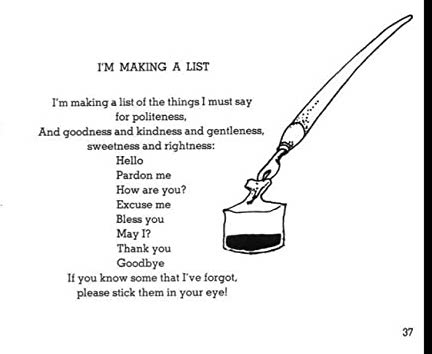
\includegraphics[width=0.5\linewidth]{images/shel_silverstein.jpg}
  \end{center}
\end{frame}

\begin{frame}{Example 1: Gentzkow and Shapiro (2010)}
  \begin{columns}[onlytextwidth, T] % align columns
    \begin{column}{.5\textwidth}
      \begin{wideitemize}
      \item How are $X_{1}$ and $X_{2}$ constructed?
        \begin{itemize}
        \item G\&S focus on highly split phrases (bigrams and trigrams) in $X_{2}$
        \item The focus is then on this set of words in $X_{1}$ and $X_{2}$
        \item Note that $y_{2}$ is not used to sign things!
        \end{itemize}
      \item Then, a \emph{supervised} measure is used to construct a
        mapping: $y_{2} = f(X_{2})$ and then applied to $X_{1}$ to
        construct $\hat{y}_{1}$
      \end{wideitemize}
    \end{column}%
    \hfill%
    \begin{column}{.5\textwidth}
      \only<1>{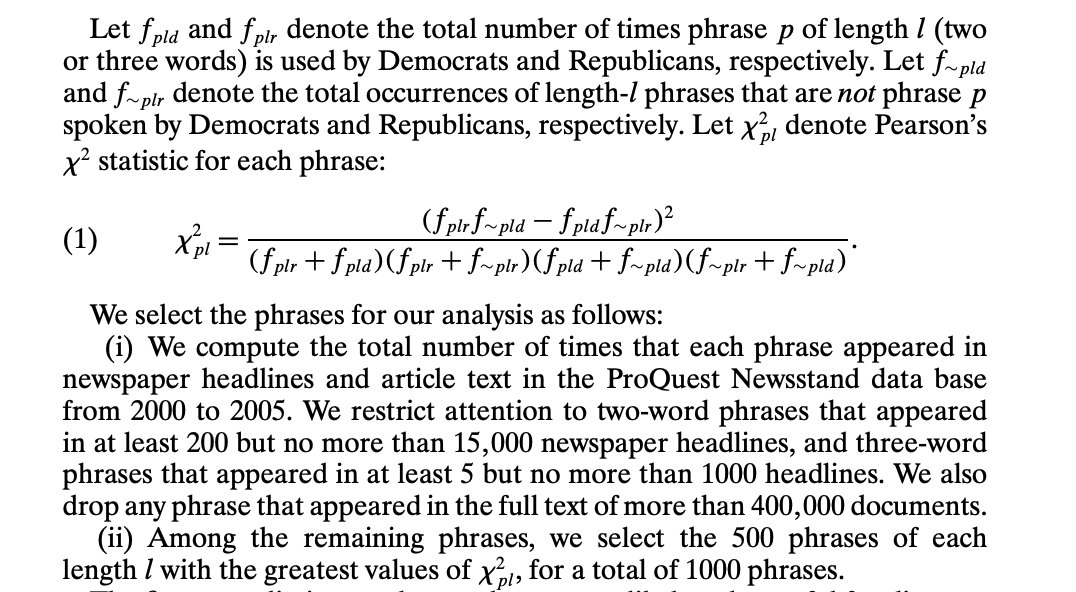
\includegraphics[width=\linewidth]{images/gentzkowshapiro_2.png}}
      \only<2>{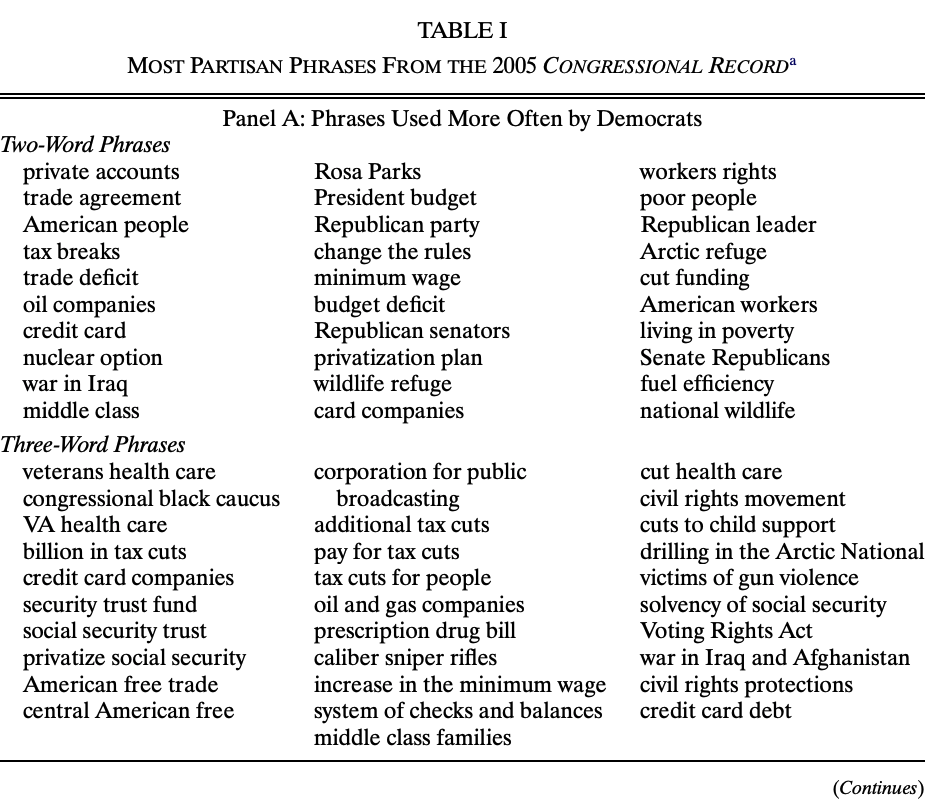
\includegraphics[width=\linewidth]{images/gentzkowshapiro_3.png}}
      \only<3>{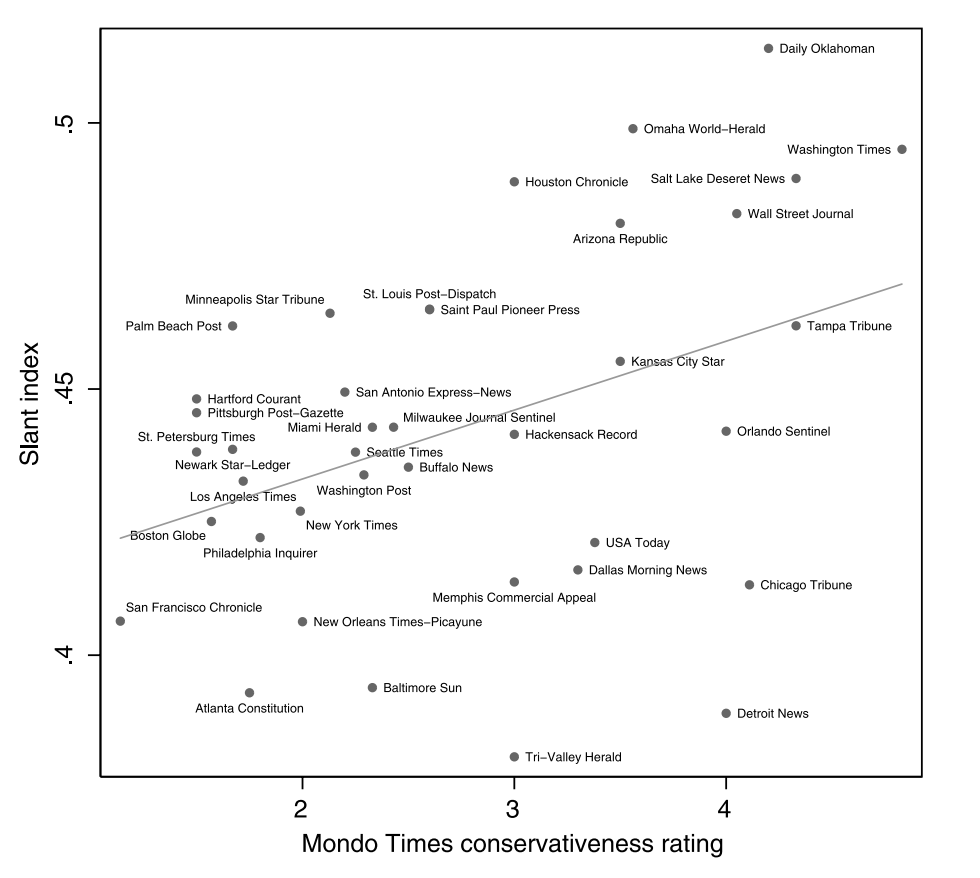
\includegraphics[width=\linewidth]{images/newspaper_slant.png}}
      \only<4>{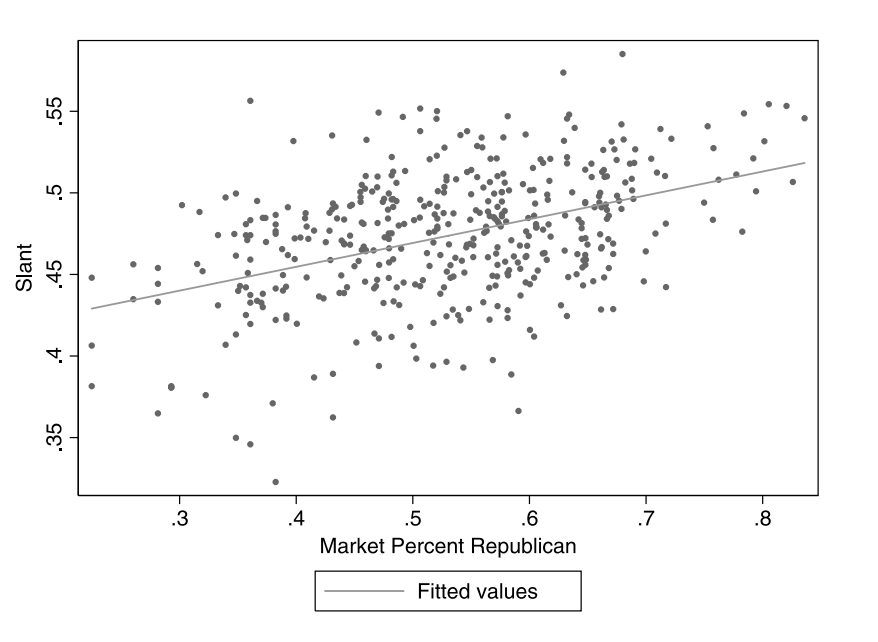
\includegraphics[width=\linewidth]{images/newspaper_slant2.png}}
    \end{column}%
  \end{columns}
\end{frame}




\begin{frame}{Example 2: Bandiera et al. (2017)}
    \begin{columns}[onlytextwidth, T] % align columns
      \begin{column}{.5\textwidth}
        \begin{wideitemize}
        \item In this example, $\mathcal{X}$ are CEO behavior at firms
          \begin{itemize}
          \item Data is converted to $X$ using diaries of activity
            which are ``coded'' using surveys
          \item ``Data on 42,233 activities of different duration,
            equivalent to 225,721 15-minute blocks, 90\% of which
            cover work activities''
          \end{itemize}
        \item This high dimensional object is then converted into a lower dimensional $\theta$, which is then correlated with firm outcomes
          \begin{itemize}
          \item The move to $\theta$ is doing dimension reduction!
          \item So how do they do it? LDA
          \end{itemize}
        \end{wideitemize}
      \end{column}%
      \hfill%
      \begin{column}{.5\textwidth}
        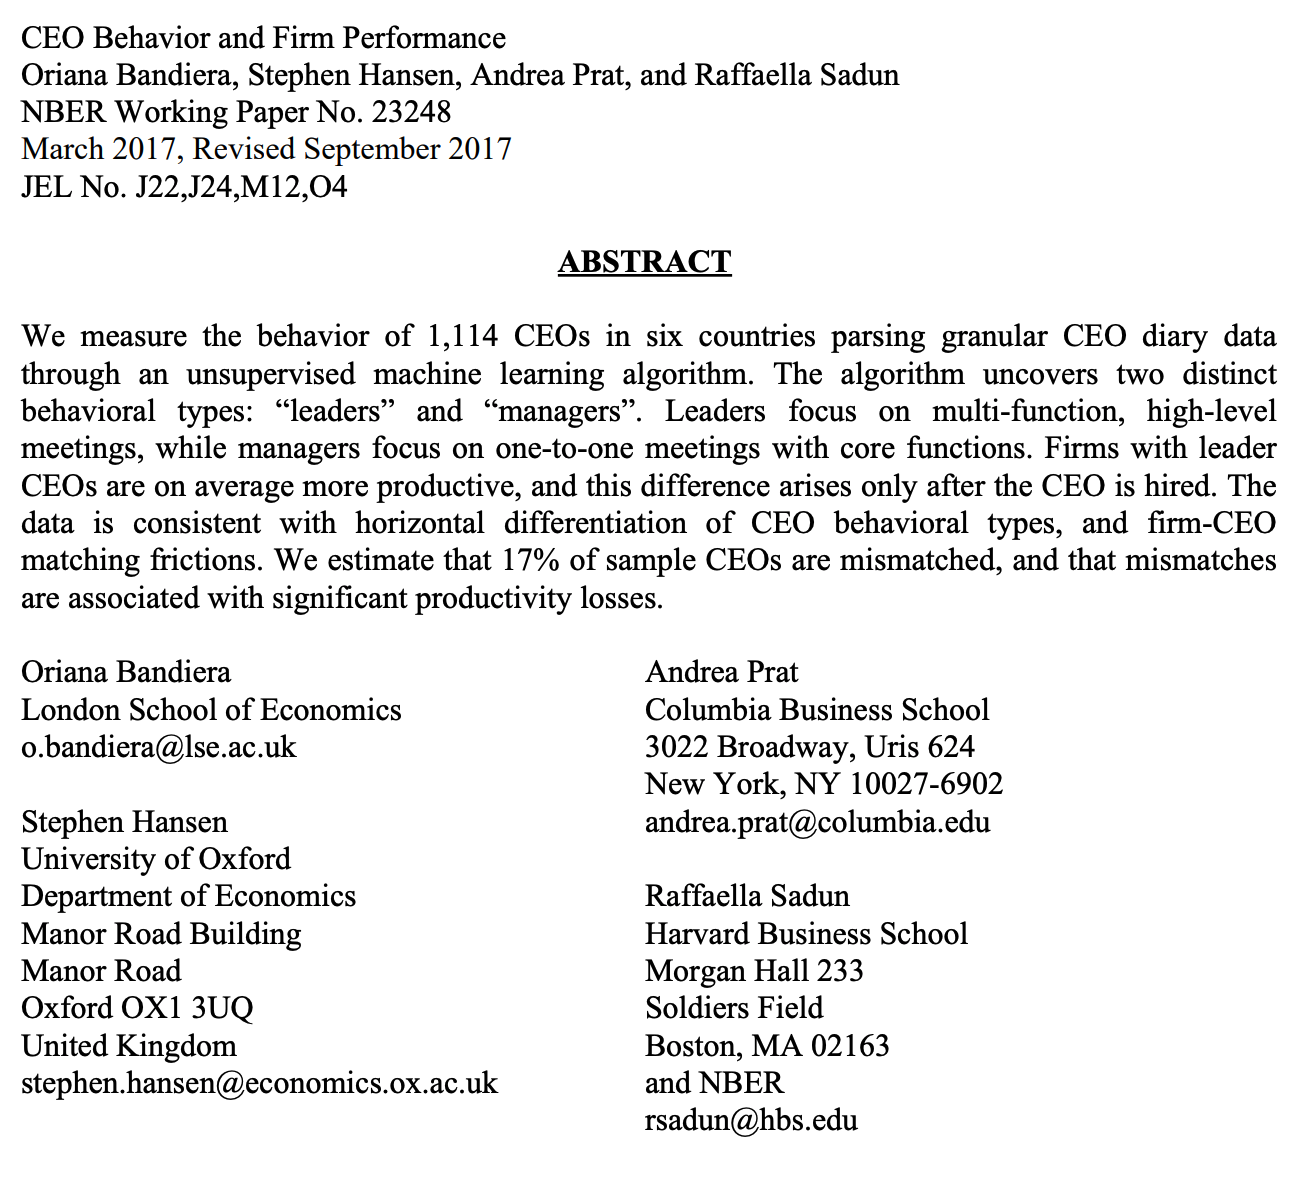
\includegraphics[width=\linewidth]{images/bandiera_1.png}
      \end{column}%
    \end{columns}
  \end{frame}

  \begin{frame}{What is LDA? Latent Dirichlet Allocation}
    \begin{columns}[onlytextwidth, T] % align columns
      \begin{column}{.5\textwidth}
        \begin{wideitemize}
        \item Originally described by Blei, Ng and Jordan (2003), LDA is a
          generative model of how a matrix of count variables, $X$, of
          dimension $n \times p$ is made
        \item $p$ is the number of potential words (or bigrams), $n$ is the
          number of documents (e.g. CEO surveys)
        \item LDA is, in essence, a structured mixture model
          \begin{itemize}
          \item Uses a Hierarchical Bayesian structure (recall our lecture!)
          \item The structure provides a way to inform structure by
            shrinking across
          \end{itemize}
        \item Assume an ``unobserved'' dimensionality 
        \end{wideitemize}
      \end{column}%
      \hfill%
      \begin{column}{.5\textwidth}
        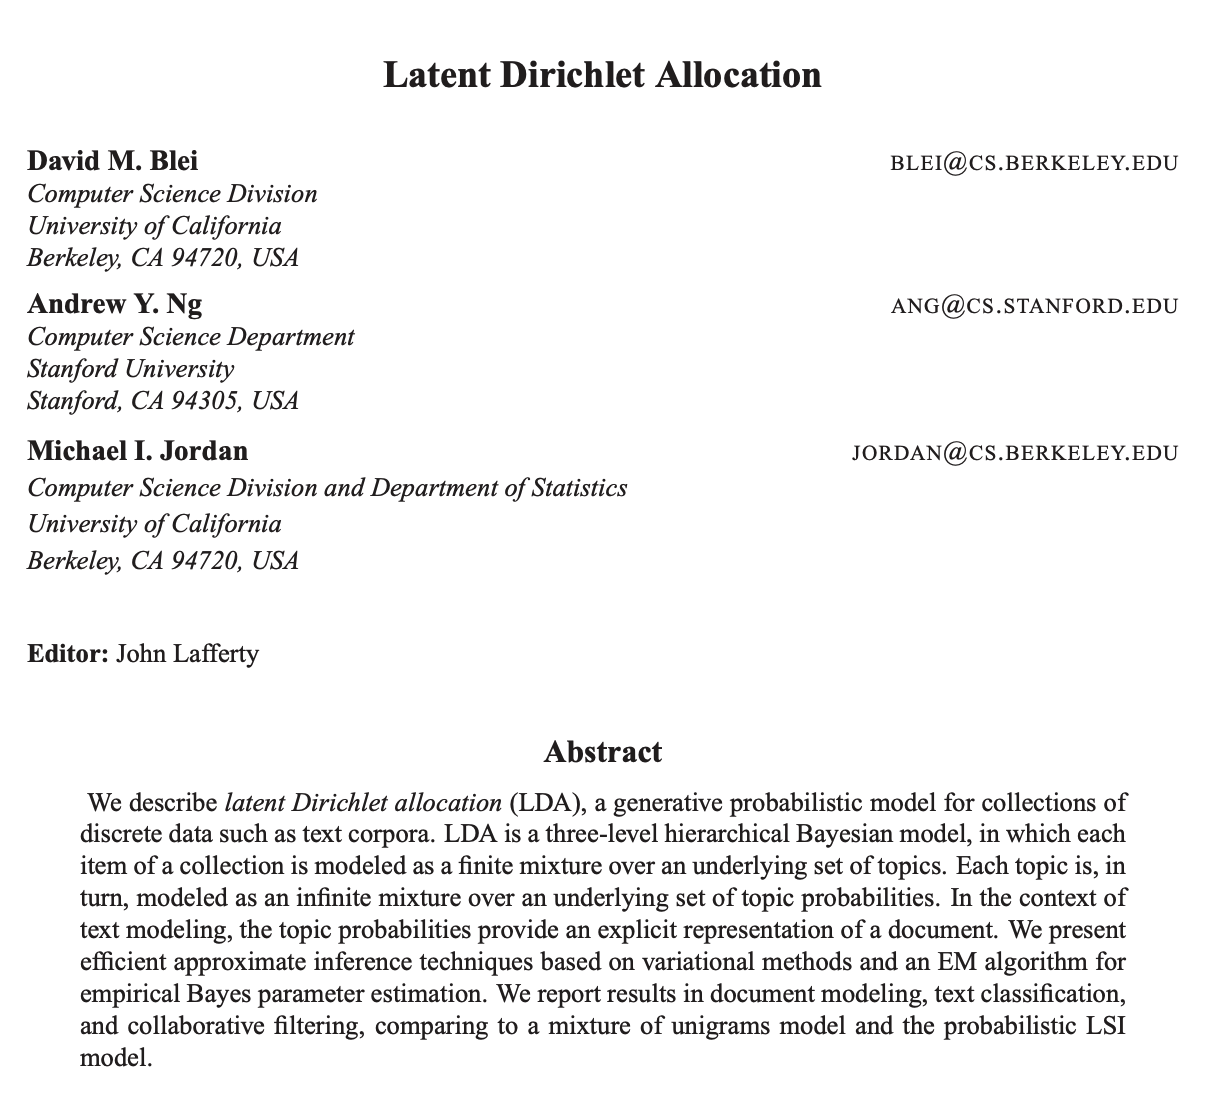
\includegraphics[width=\linewidth]{images/blei_1.png}
      \end{column}%
    \end{columns}
  \end{frame}

  \begin{frame}{What is LDA? Latent Dirichlet Allocation}
    \begin{columns}[onlytextwidth, T] % align columns
      \begin{column}{.5\textwidth}
        \begin{wideitemize}
        \item Simple example from Bandiera et al.: there are two types
          (e.g. unobserved dimension of 2)
          \begin{itemize}
          \item All CEOs are drawn from one of two types            
          \end{itemize}
        \item Consequentially, LDA model will estimate:
          \begin{itemize}
          \item For a given CEO, what is the probability that they are type 1 or type 2 (0 or 1)
          \item For each type, what is the relative distribution of each activity
          \end{itemize}
        \end{wideitemize}
      \end{column}%
      \hfill%
      \begin{column}{.5\textwidth}
        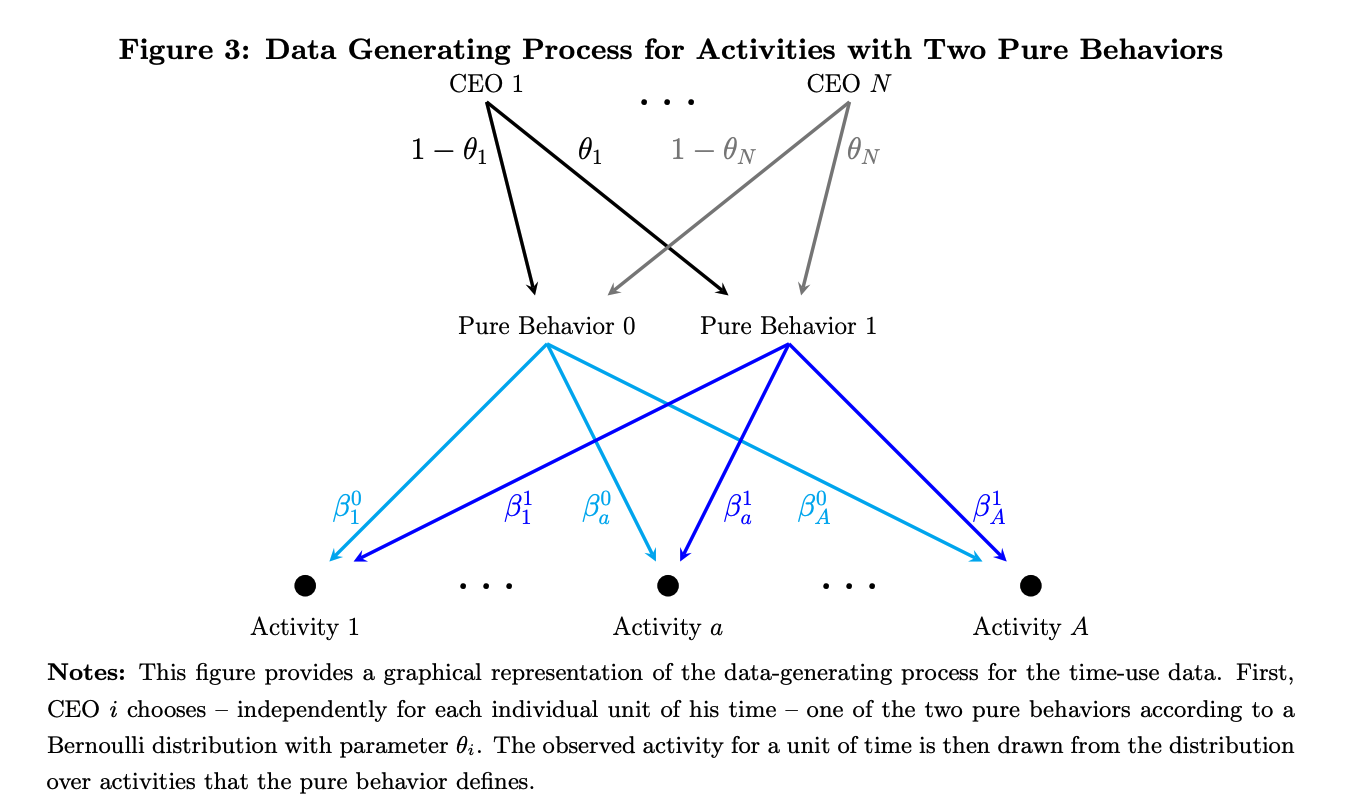
\includegraphics[width=\linewidth]{images/bandiera_2.png}
      \end{column}%
    \end{columns}
  \end{frame}

  \begin{frame}{What is LDA? Latent Dirichlet Allocation}
    \begin{columns}[onlytextwidth, T] % align columns
      \begin{column}{.5\textwidth}
        \begin{wideitemize}
        \item Output of this model gives a number of pieces: for each
          CEO, we have an measure of how much they are each type
        \item For each activity, we know how much they reflect each
          ``type''
        \item For Bandiera et al., they use the type measure
          ($\theta$), as an index
        \end{wideitemize}
      \end{column}%
      \hfill%
      \begin{column}{.5\textwidth}
        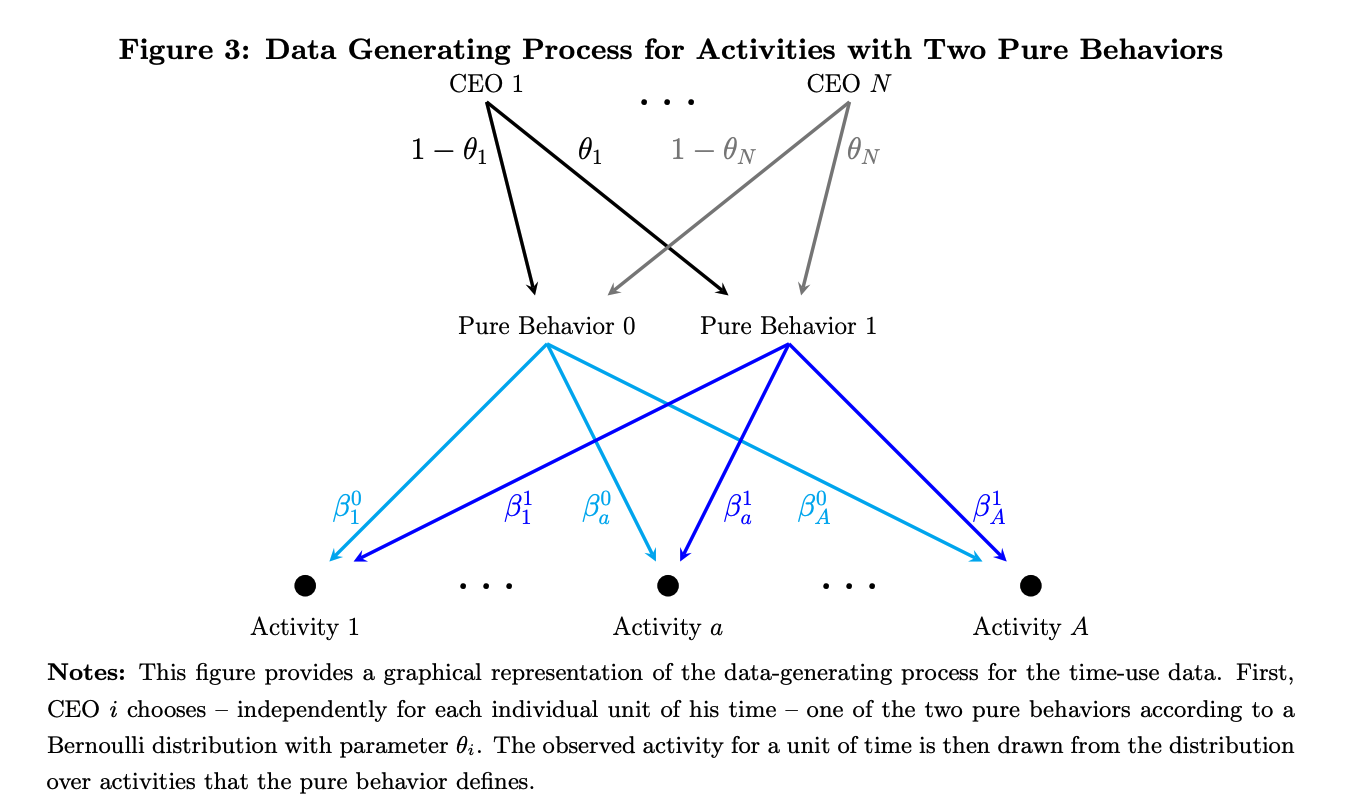
\includegraphics[width=\linewidth]{images/bandiera_2.png}
      \end{column}%
    \end{columns}
  \end{frame}

  \begin{frame}{The issues or challenges with LDA}
    \begin{wideitemize}
    \item What do the types even mean?
      \begin{itemize}
      \item E.g. what is type 1? What is type 2?
      \end{itemize}
    \item Why is 2 the right number?
      \begin{itemize}
      \item Consider the analogy to Principal Component Analysis
      \item Dimension choice can be done using maximum Bayes Factor
        (see Bybee et al. (2020))
      \end{itemize}
    \item There are a number of ways to diagnose the types:
      \begin{itemize}
      \item Correlate them with some other label from outside the data
      \item Subjectively label them by examining the $\beta$ frequencies for each document
        \begin{itemize}
        \item E.g. if one type puts a lot on one type of activity, you could construct a name for it
        \item This is just correlating using the human mind
        \end{itemize}
      \end{itemize}
    \end{wideitemize}
  \end{frame}


  \begin{frame}{The issues or challenges with LDA}
    \begin{columns}[onlytextwidth, T] % align columns
      \begin{column}{.5\textwidth}
    \begin{wideitemize}
    \item This model is Bayesian, and uses priors to initialize the model
    \item It turns out that the parameters of the model are
      unidentified, generically
      \begin{itemize}
      \item The joint probability of the corpus from model is given by
        $P = B\Theta$, where $B$ is the matrix of $\beta$
        ($p \times K$), and $\Theta$ is $K \times n$
      \item Concretely, imagine $p = 1$, and $K = 2$
      \end{itemize}
    \item The priors are necessary for estimation!
      \begin{itemize}
      \item As a result, choice of prior can move your results
      \item Many empiricists might feel uncomfortable with this        
      \end{itemize}
    \end{wideitemize}
      \end{column}%
      \hfill%
      \begin{column}{.5\textwidth}
        \only<1->{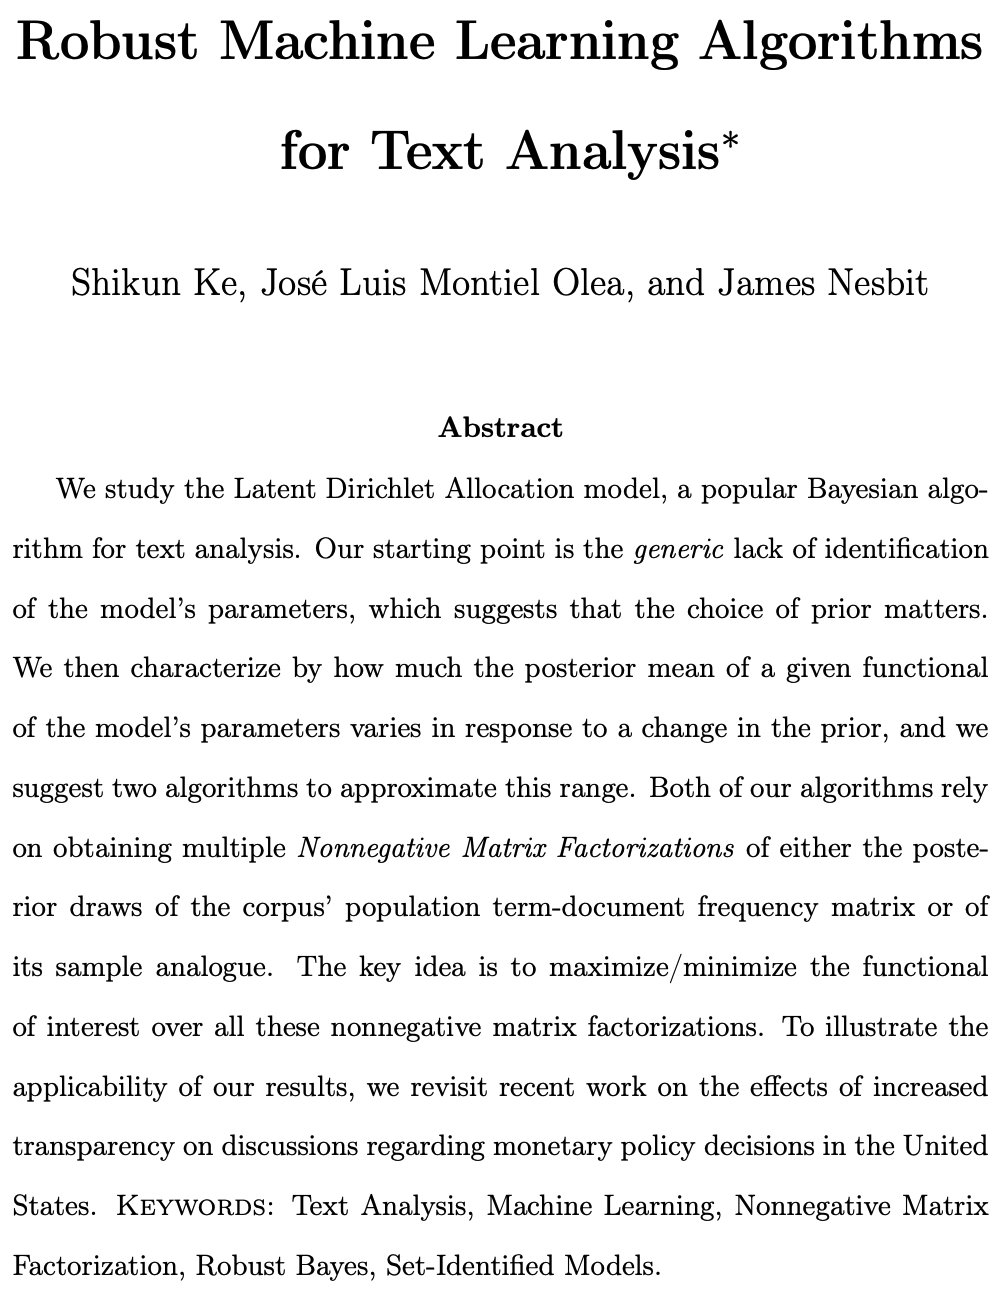
\includegraphics[width=\linewidth]{images/pepe_1.png}}
        \only<2->{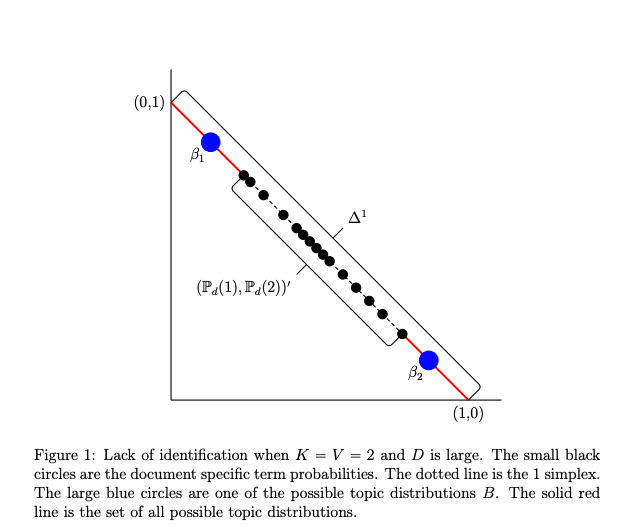
\includegraphics[width=\linewidth]{images/lda_unidentified.png}        }
      \end{column}%
    \end{columns}
  \end{frame}

  \begin{frame}{Example 3: TFIDF + Cosine Similarity}
    \begin{columns}[onlytextwidth, T] % align columns
      \begin{column}{.5\textwidth}
        \begin{wideitemize}
        \item Define a concept called TFIDF: term-frequency inverse document frequency
          \begin{equation}
            TF_{pw} = \frac{c_{pw}}{\sum_{k}c_{pk}}
          \end{equation}
          which is the frequency that word $w$ shows up in document $p$ relative to the other words.
        \item Define $IDF_{w}$ as
          \begin{equation}
            IDF_{w} = \log\left(\frac{d}{d \text{with word } w}\right)
          \end{equation}
        \item $TFIDF_{pw}$ is  the product of those two.
        \end{wideitemize}
      \end{column}%
      \hfill%
      \begin{column}{.5\textwidth}
        \only<1->{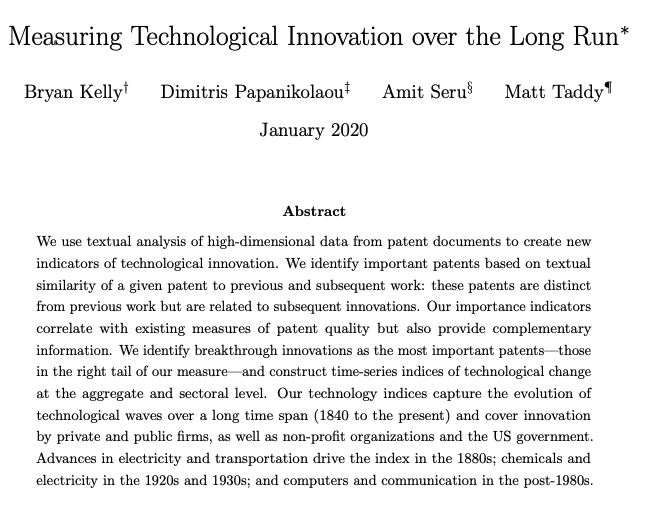
\includegraphics[width=\linewidth]{images/kelly_cosine.png}}
      \end{column}%
    \end{columns}
  \end{frame}

  \begin{frame}{Example 3: TFIDF + Cosine Similarity}
    \begin{columns}[onlytextwidth, T] % align columns
      \begin{column}{.5\textwidth}
        \begin{wideitemize}
        \item This paper constructs BIDF, which is a backwards looking version of IDF:
          \begin{equation}
            \tiny IDF_{wp} = \log\left(\frac{\text{patents priors to p}}{\text{1+ patents prior to p that include w}}\right)
          \end{equation}
        \item Finally, they look at the cosine distance between these TFBIDF for a given patent.
          \item They can identify ``new'' patents using this!
        \end{wideitemize}
      \end{column}%
      \hfill%
      \begin{column}{.5\textwidth}
        \only<1->{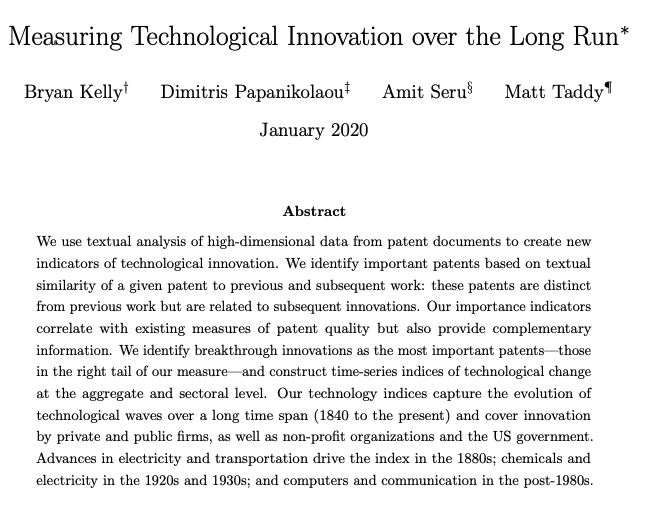
\includegraphics[width=\linewidth]{images/kelly_cosine.png}}
      \end{column}%
    \end{columns}
  \end{frame}


  \begin{frame}{Example 4: Using LLMs to construct new data}
    \begin{columns}[onlytextwidth, T] % align columns
      \begin{column}{.5\textwidth}
       \only<1-4>{ \begin{wideitemize}
        \item Since the advent of ChatGPT (and other LLMs), there has been a huge push to use these models to construct new data
        \item Some examples:
  \begin{itemize}
    \item Construct beliefs (Bybee (2024))
    \item Simulate experiments (Horton (2024))
    \item Classify documents 
    \item Embed characteristics
  \end{itemize}        
  \item Bybee (2024) uses ChatGPT to elicit beliefs about macroeconomic conditions using news articles
  \begin{itemize}
    \item ChatGPT's elicited beliefs are much like surveyed beliefs, not objective!
  \end{itemize}
        \end{wideitemize}}
\only<5>{\begin{wideitemize}
  \item Outstanding statistical problems:
  \begin{itemize}
    \item How do we think about uncertainty?
    \item How do we think about memorization?
  \end{itemize}
\end{wideitemize}
}
\end{column}%
      \hfill%
      \begin{column}{.5\textwidth}
        \only<1>{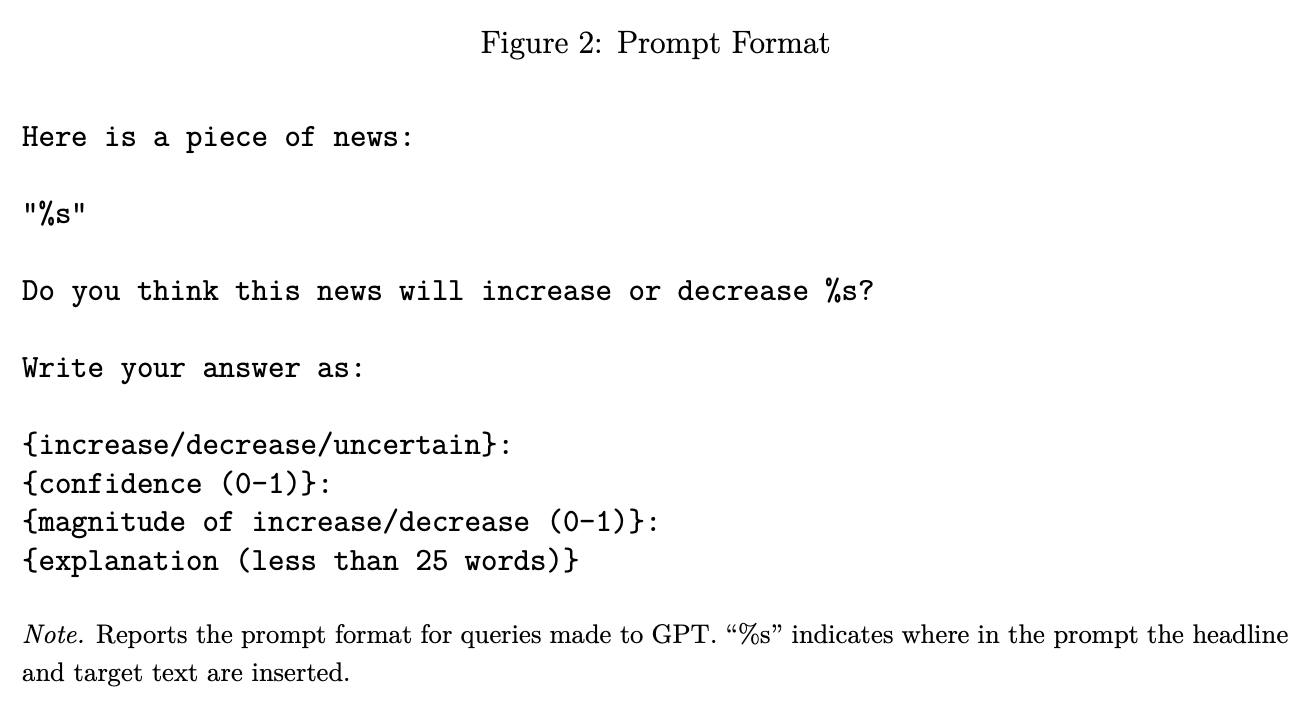
\includegraphics[width=\linewidth]{images/bybee1.png}}
        \only<2>{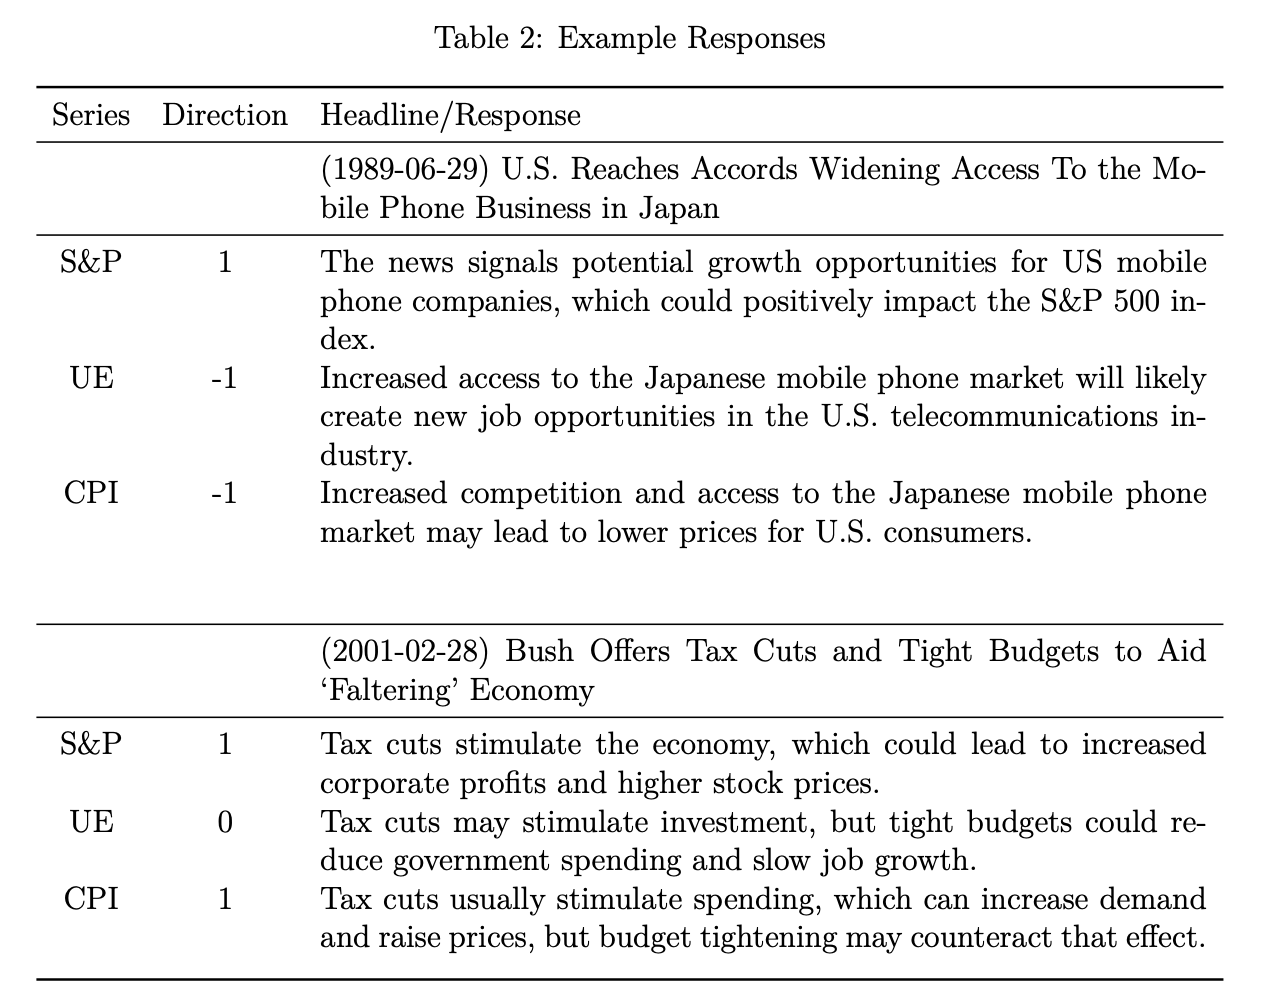
\includegraphics[width=\linewidth]{images/bybee2.png}}
        \only<3>{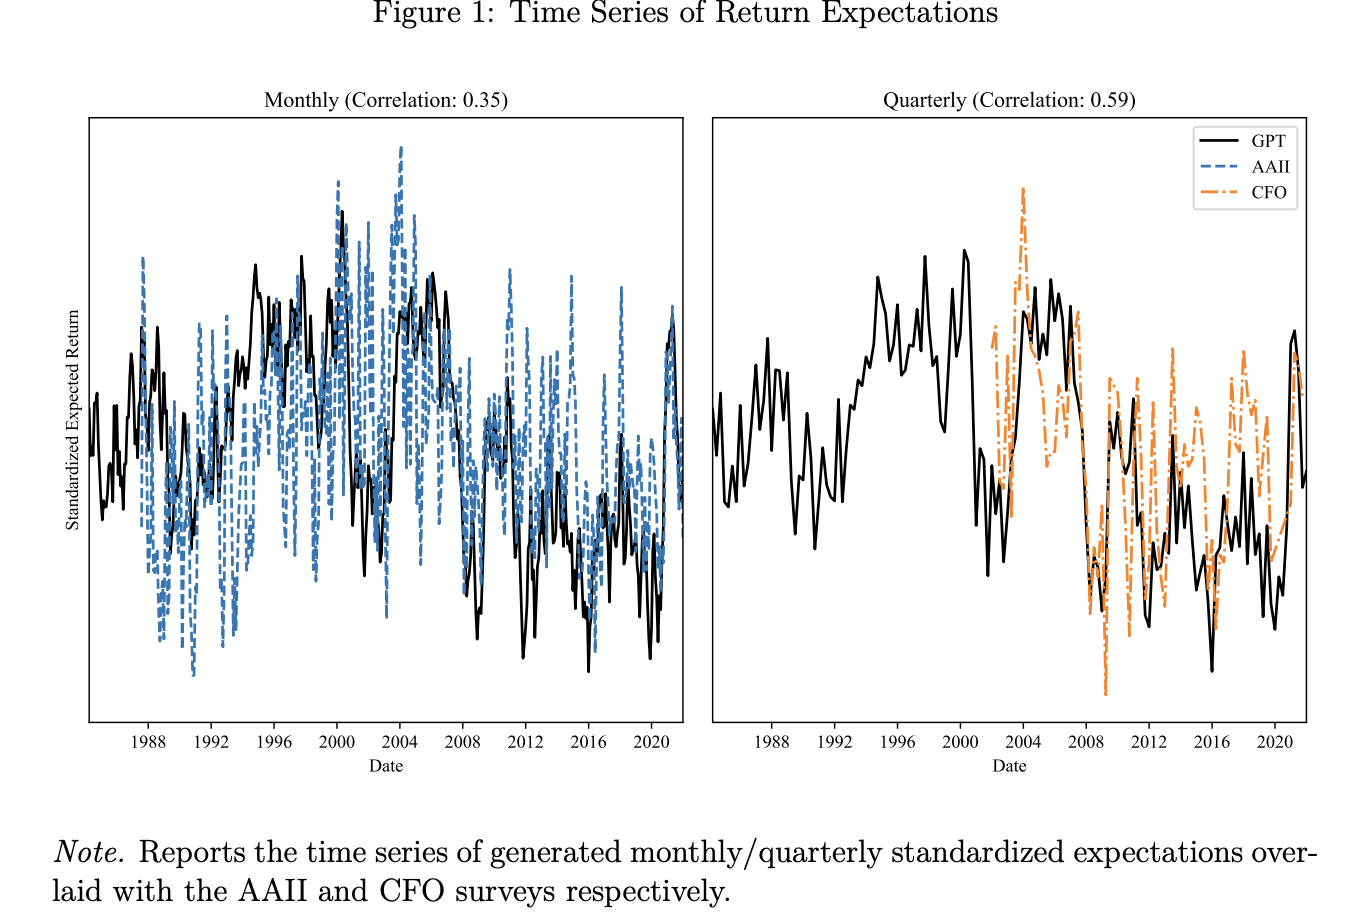
\includegraphics[width=\linewidth]{images/bybee3.png}}
        \only<4->{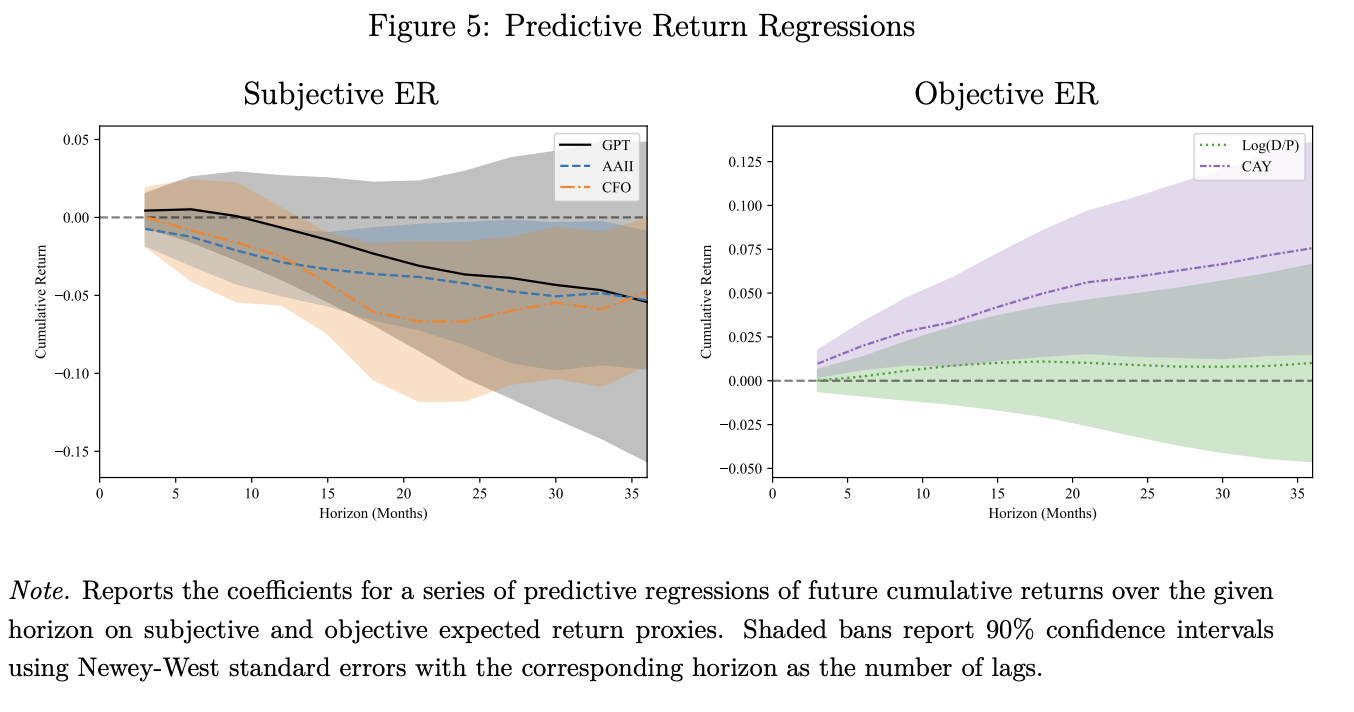
\includegraphics[width=\linewidth]{images/bybee4.png}}
      \end{column}%
    \end{columns}
  \end{frame}



%   \begin{frame}{Example 5: Embedding characteristics for comparisons}
%     \begin{columns}[onlytextwidth, T] % align columns
%       \begin{column}{.5\textwidth}
%  \begin{wideitemize}
%         \item Embeddings are a way to convert words into a continuous space
%         \end{wideitemize}
% \end{column}%
%       \hfill%
%       \begin{column}{.5\textwidth}
%         \only<1>{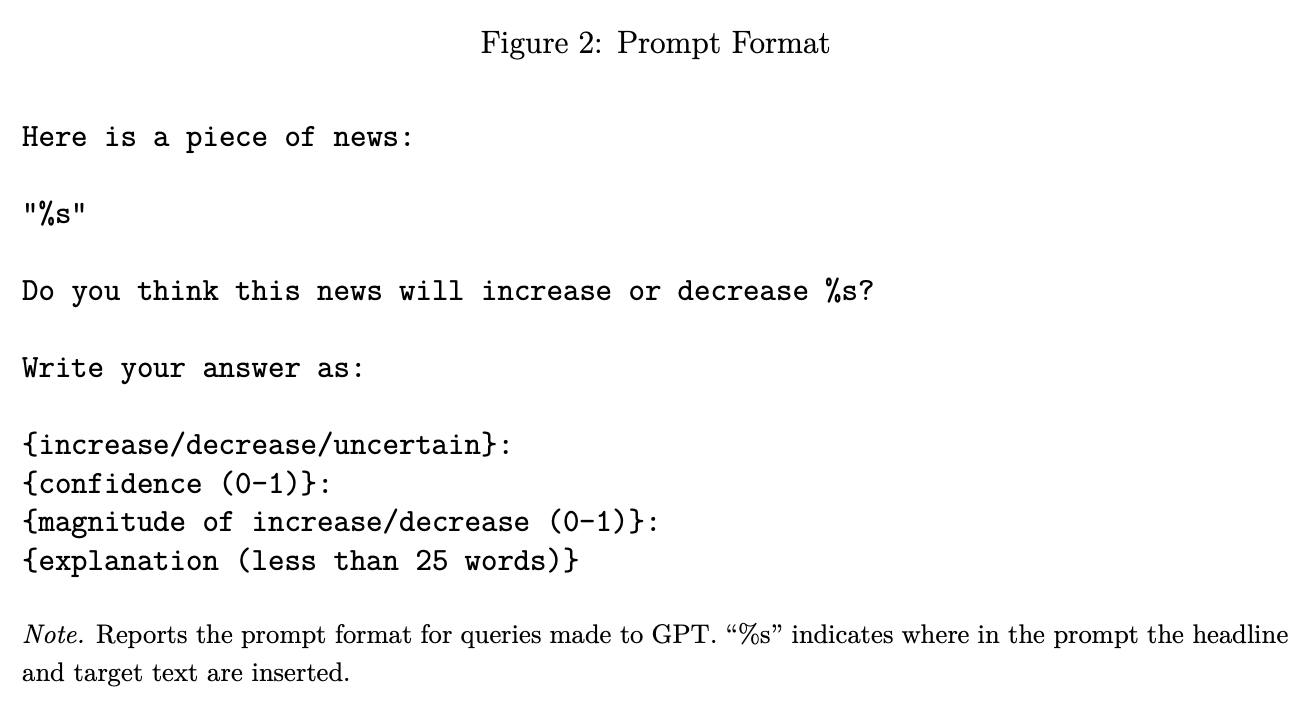
\includegraphics[width=\linewidth]{images/bybee1.png}}
%       \end{column}%
%     \end{columns}
%   \end{frame}
  
  
  \begin{frame}{My Main takeaway}
    \begin{wideitemize}
    \item This is a really powerful way to take new data and apply to problems
    \item However, really easy to parse and summarize data without a good economic question in mind
      \begin{itemize}
      \item Still need exogeneous variation and an economic question!
      \end{itemize}
    \item Without a research design in mind, it becomes very hard to
      describe ``why'' you're doing something.
      \begin{itemize}
      \item Personal expereince with my own work
      \end{itemize}
    \item Advent of LLMs has opened up this space tremendously
    \end{wideitemize}
  \end{frame}
\end{document}